\documentclass[%margin%,line,pifont,palatino,courier
]{article}
\usepackage{fullpage}
\usepackage{lastpage}
\usepackage[top=1in,bottom=1in,margin=1in]{geometry}
\usepackage{supertabular}
\usepackage{graphicx,tikz}	
%\usepackage{tkz-euclide}
%\usetkzobj{all}
%\usetikzlibrary{calc}
\usepackage{array,multicol}
\usepackage{amsmath,amssymb}
\usepackage{enumitem}
%\usepackage{framed}

\usepackage{fancyhdr}
\pagestyle{fancy}

\addtolength{\topmargin}{-0.25in}

\newcommand{\vect}[1]{\mathbf{#1}}
\DeclareMathOperator{\proj}{proj}

\fancypagestyle{plain}{
	\addtolength{\headheight}{0.485in}
	\rhead{\bf MATH 2574 (Calculus III) \\
		%\vspace{0.5pc}
		%due Fri 10 Mar 
		Spring 2017 \\}
	\rfoot{\footnotesize $\;$Quiz 5TH, p. \thepage\ (of \pageref{LastPage})
	}
\renewcommand{\headrulewidth}{0pt}
}
\fancyhf{}
\renewcommand{\headrulewidth}{0pt}
\rfoot{\footnotesize Quiz 5TH, p. \thepage\ (of \pageref{LastPage})$\;$}

\title{\vspace{-3.5pc} 
	\flushleft \bf \Large Take-Home Quiz 5: Miscellaneous \\ (\S 10.1-10.3, 12.3, 12.6-12.7, 13.1, 13.5)}
\date{}

% % % % %
\begin{document}
\maketitle

\vspace{-3pc}
%\noindent{\bf Directions:} This quiz is due on March 3, 2017 at the beginning of lecture.  You may use whatever resources you like -- e.g., other textbooks, websites, collaboration with classmates -- to complete it \textbf{but YOU MUST DOCUMENT YOUR SOURCES}.  Acceptable documentation is enough information for me to find the source myself.  Rote copying another's work is unacceptable, regardless of whether you document it.  

\noindent\hrulefill

\begin{enumerate}

% % %
\item {\bf 10.1 \#74}
Match equations (a)-(d) with graphs (A)-(D).  Explain your reasoning.
\begin{enumerate}
\item $x=t^2-2,\,y=t^3-t$
\item $x=\cos{(t+\sin{50t})},\,y=\sin{(t+\cos{50t})}$
\item $x=t+\cos{2t},\,y=t-\sin{4t}$
\item $x=2\cos t+\cos{20t},\,y=2\sin t+\sin{20t}$
\end{enumerate}
%\vspace{1pc}

\begin{center}
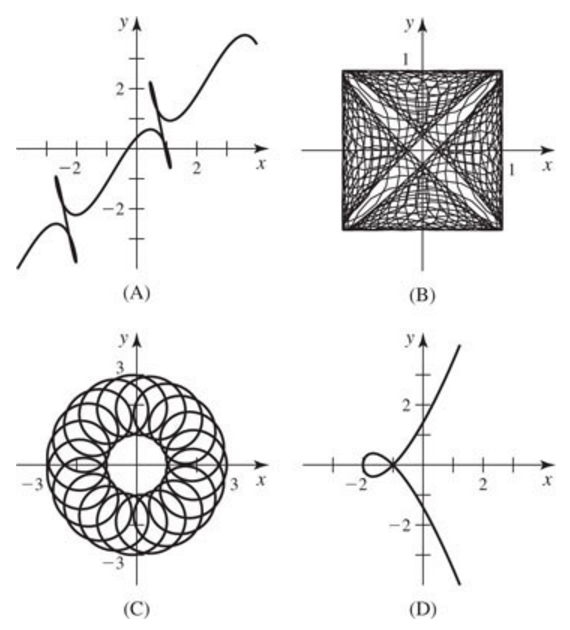
\includegraphics[scale=0.75]{THQ510-1}
\end{center}

% % %
\item {\bf 10.3 \#16, 18, 20}
Find the points at which the following polar curves have a horizontal or a vertical tangent line.
\begin{enumerate}
\item $r=2+2\sin{\theta}$
\item $r=3+6\sin{\theta}$
\item $r=\sec{\theta}$
\end{enumerate}

% % %
\item {\bf 12.3 \#74}
Find the value of $a$ for which $f$ is continuous at all points in $\mathbb R^2$.
\[
f(x,y)=\begin{cases} \dfrac{1+2xy-\cos{xy}}{xy} & \text{if }xy\neq 0 \\
	a & \text{if }xy=0
	\end{cases}
\]

% % %
\item {\bf 13.1 \#52}
Find the value of $a>0$ such that the average value of the function
\[
f(x,y)=x+y-8
\]
over the region $R=\{(x,y)\mid 0\leq x\leq a,\,0\leq y\leq a\}$ is zero.

\newpage
% % %
\item {\bf 10.2 \#89}
The equations
\[
r=a+b\cos{\theta}\qquad\text{and}\qquad r=a+b\sin{\theta}
\]
describe curves known as \textbf{lima\c cons}.
\begin{itemize}
\item If $|a|=|b|$ then the lima\c con is a \textbf{cardiod}.
\item If $|a|<|b|$ then the lima\c con has an inner loop. 
\item If $|b|<|a|<2|b|$ then the lima\c con has a dent or dimple.
\item If $|a|>2|b|$ then the lima\c con is oval-shaped.
\end{itemize}
Match equations (a)-(f) with the lima\c cons in figures (A)-(F).
\begin{enumerate}
\item $r=-1+\sin{\theta}$
\item $r=2+\sin{\theta}$
\item $r=1+2\sin{\theta}$
\item $r=-1+2\cos{\theta}$
\item $r=1-2\cos{\theta}$
\item $r=1+\frac{2}{3}\sin{\theta}$
\end{enumerate}

\begin{center}
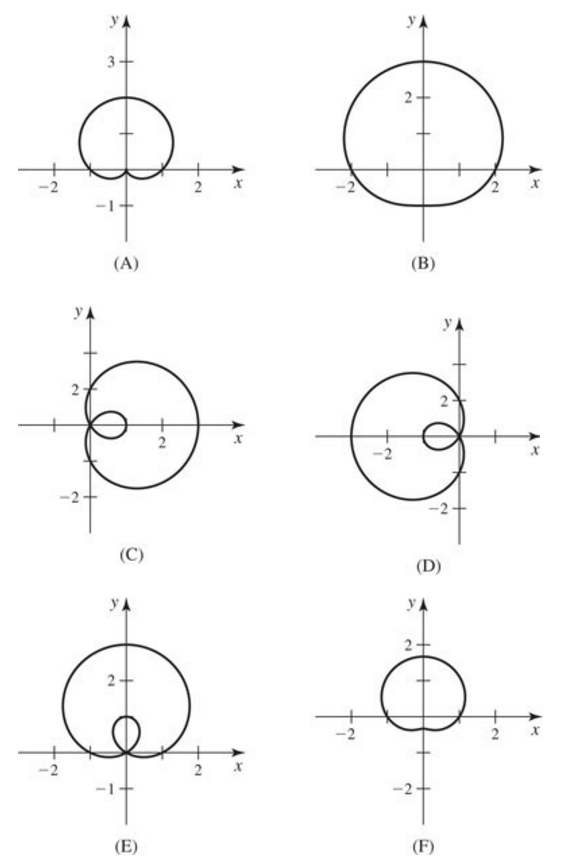
\includegraphics[scale=0.9]{THQ510-2}
\end{center}

% % %
\item {\bf 12.6 \#48}
Consider the upper half of the ellipsoid
\[
f(x,y)=\sqrt{1-\dfrac{x^2}{4}-\dfrac{y^2}{16}}
\]
and the point $P=(0,\sqrt 8)$ given on the level curve $f(x,y)=\frac{1}{\sqrt 2}$.  Compute the slope of the line tangent to the level curve at $P$ and verify that the tangent line is orthogonal to the gradient at that poitnt.

% % %
\item {\bf 12.7 \#18}
Find an equation of the plane tangent to the surface
\[
z=2+2x^2+\dfrac{y^2}{2}
\]
at the point $(-\frac{1}{2},1,3)$.  Sketch the surface along with the tangent plane.

% % %
\item {\bf 12.7 \#36}
The volume of a right circular cone with radius $r$ and height $h$ is $V=\dfrac{\pi r^2h}{3}$.  Use linear approximation to:
\begin{enumerate}
	\item approximate the change in the volume of the cone when the radius changes from $r=6.5$ to $r=6.6$ and the height changes from $h=4.20$ to $h=4.15$.
	\item approximate the change in volume of the cone when the radius changes from $r=5.40$ to $r=5.37$ and the height changes from $h=12.0$ to $h=11.96$.
\end{enumerate}

% % %
\item {\bf 13.5 \#50, 52}
Find the volume of the following solids:
\begin{enumerate}
	\item the solid bounded by the cylinders $r=1$ and $r=2$ and the cones $\varphi=\frac{\pi}{6}$ and $\varphi=\frac{\pi}{3}$. 
	
	\begin{center}
	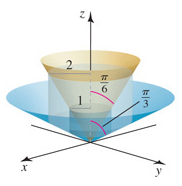
\includegraphics[scale=1]{13-5no50}
	\end{center}
	
	\item the solid inside the cone $z=\sqrt{x^2+y^2}$ that lies between the planes $z=1$ and $z=2$.
	
	\begin{center}
	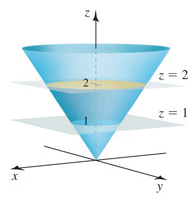
\includegraphics[scale=1]{13-5no52}
	\end{center}
	
\end{enumerate}

% % % % %
\end{enumerate}
\end{document}